\documentclass[a4paper,12pt,oneside,openany]{article}
\usepackage{cmap}
\usepackage[utf8]{inputenc}
\usepackage{lmodern}
\usepackage[T1]{fontenc}
\usepackage[english]{babel}
\usepackage{pdfpages}
\usepackage{fontenc}
\usepackage{bibunits}
\usepackage{etoolbox}
\apptocmd{\thebibliography}{\raggedright}{}{}
\begin{document}
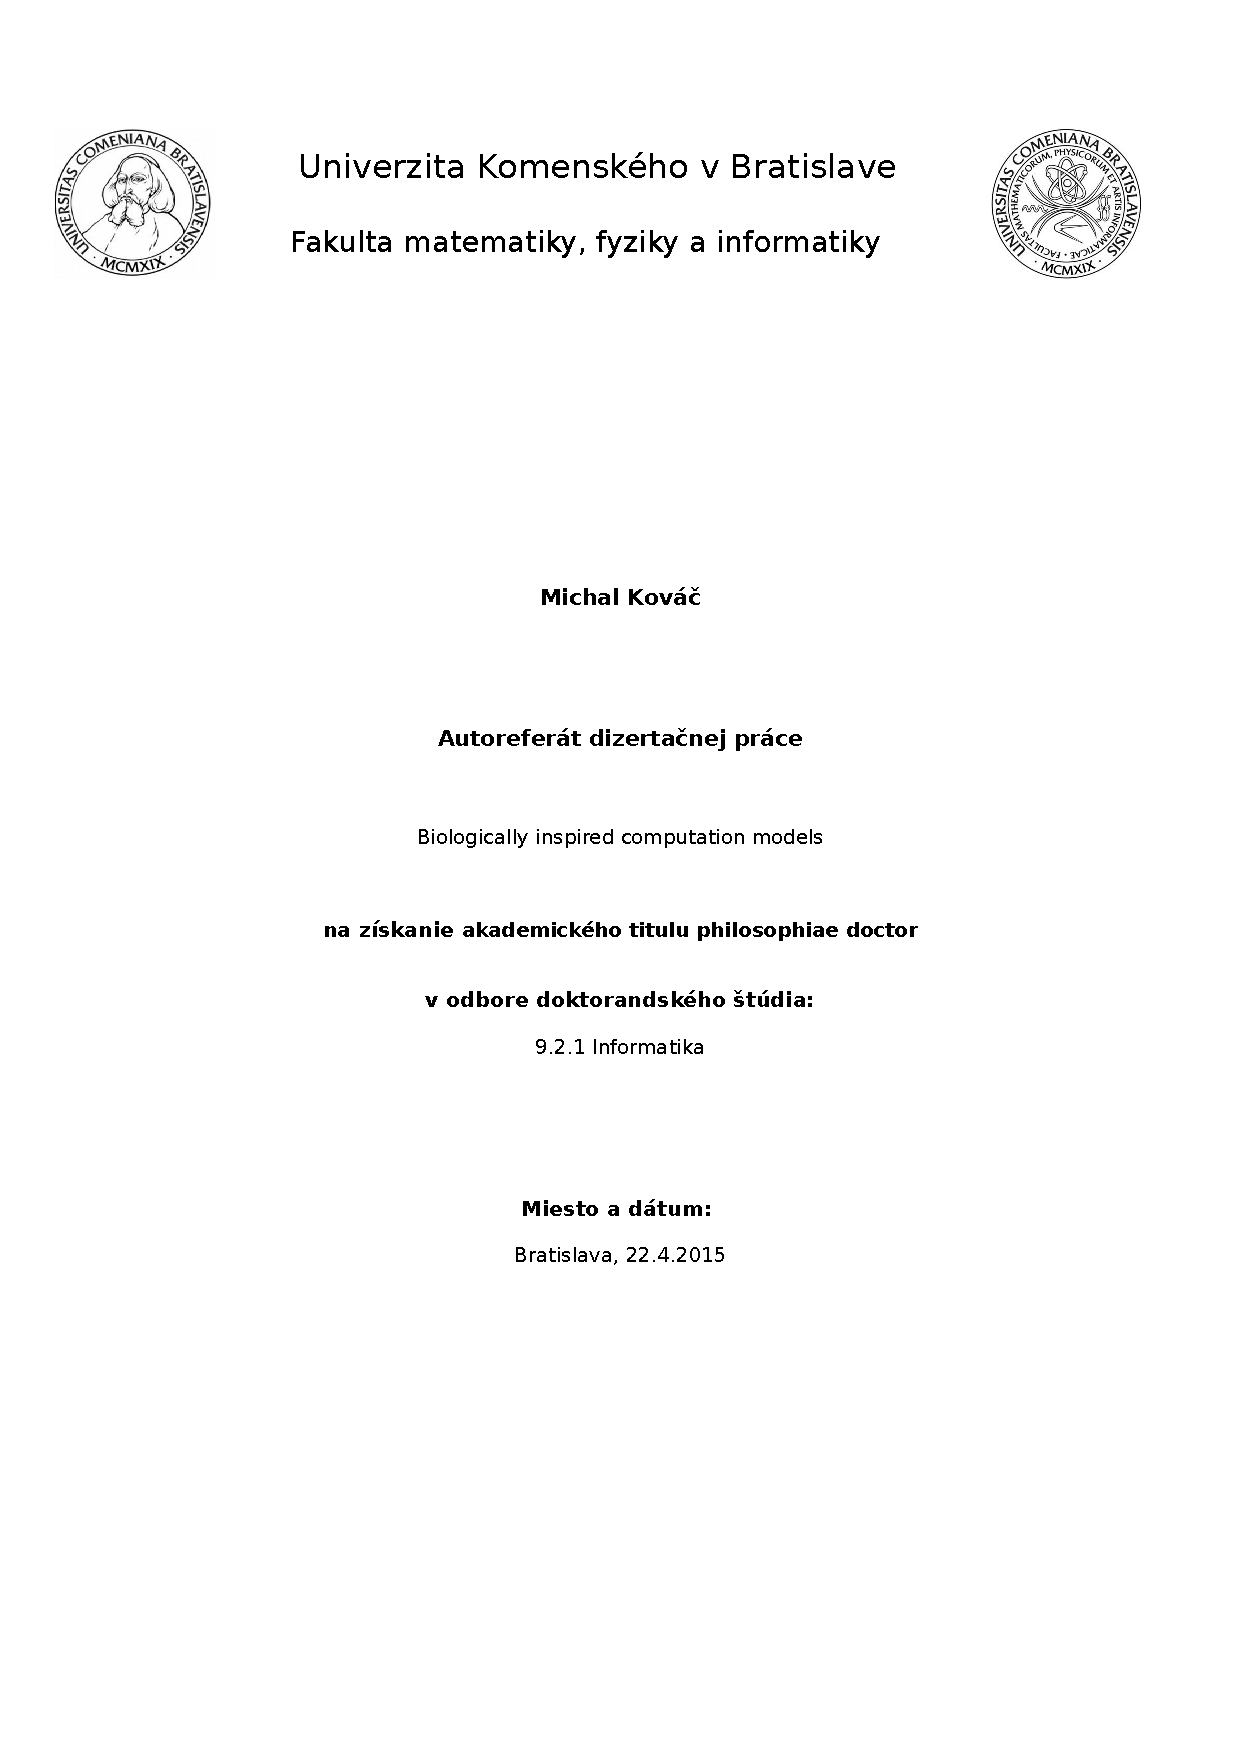
\includepdf[pages={1,2}]{autoreferat_template.pdf}

\section*{Introduction}
There are a lot of areas in the theoretical computer science that are
motivated by other science fields. Computation models motivated by
biology forms a large group of them. They include neural networks,
computational models based on DNA evolutionary algorithms, which
have already found their use in computer science and proved that it is
worth to be inspired by biology. L-systems are specialized for describing
the growth of plants, but they have also found the applications in
computer graphics, especially in fractal geometry.

Other emerging areas are still awaiting for their more significant uses.
One of them is the membrane computing. It is relatively young field of
natural computing - in comparison: neural networks have been
researched since 1943 and membrane systems since 1998. Membrane
systems (P systems) are distributed parallel computing devices inspired
by the structure and functionality of cells. Recently, many P system
variants have been developed in order to simulate the cells more
realistically or just to improve the computational power.

\section*{P systems}
Nature computes not only at the neural or genetic level, but also at the
cellular level. In general, any non-trivial biological system has a
hierarchical structure where objects and information flows between
regions, what can be interpreted as a computation process.

The regions are typically delimited by various types of membranes at
different levels from cell membranes, through skin membrane to virtual
membranes which delimits different parts of an ecosystem. This
hierarchical system can be seen in other field such as distributed
computing, where again well delimited computing units coexist and are
hierarchically arranged in complex systems from single processors to the
internet. Membranes keep together certain chemicals or information and
selectively determines which of them may pass through.

From these observations, Păun introduces the notion of a membrane
structure as a mathematical representation of hierarchical architectures
composed of membranes. It is usually represented as a Venn diagram
with all the considered sets being subsets of a unique set and not
allowed to be intersected. Every two sets are either one the subset of the
other, or disjoint. Outermost membrane (also called skin membrane)
delimits the finite “inside” and the infinite “outside”.

\section*{Results}
We have studied several variants of sequential P systems in order to
obtain universality without using maximal parallelism. A variant with
rewriting rules that can use inhibitors was shown to be universal in both
generating and accepting case. The generating model is able to simulate
maximal parallel P system and the accepting model can simulate a
register machine. The constructive proof for the generating case is
valuable not only for the universality, but also can be seen as a method
of conversion between P systems in sequential manner and maximally
parallel manner, which may be essential for future works on P systems
and other multiset rewriting systems. Sequential variants are promising
alternative to traditional maximal parallel variants and will be good
subject for the further research. Future plans include research of other
more restricted variants such as omitting cooperation in the rules or
restricting the power of inhibitors.

In addition, we have defined a new variants of zero-testing, aiming to fit
in layers between mere reformulations of the basic sequential P system
and universal sequential P systems with inhibitors. These include various
forms of detection of empty membranes, which is specific for membrane
systems. As for now, the work is currently in progress, and the results
obtained so far have been just the computational completeness.
However, one variant with objects avoiding empty regions is more
promising for our goal because the standard contruction of register
machine do not work. We conjecture this variant is not universal, possibly
equivalent with Petri nets.

There are many features not yet combined, so we suggest them for the
fur ther research (non-cooperative rules, rules with priorities, decaying
objects, deterministic steps, ... ).

Aside from the research of the computational power, there are many
open problems in the area of decision problems of certain properties.
Interesting ideas for future work can be taken from Bottoni et. al. as they
define an abstract notion of negative application conditions for general
rewriting systems, which is for multiset rewriting rendered as usage of
inhibitors. Although they considered only nondeleting rules (after
application of each rule the resulting multiset is a superset of the current
multiset), interesting results was shown that the termination of rewriting
was shown to be decidable.

We have investigated the decidability problems of existence of (in)finite
computation for a universal class of P systems with active membranes.
We have shown and published our results that are on both sides of the
decidability barrier. Regarding the open problem stated in about
sequential active P systems with hard membranes (without
communication between membranes), it could be interesting to find a
connection between the universality and decidability of these termination
problems.

We research sequential P systems with active membranes also in
combination with notions inspired by reaction systems, i.e. using sets
instead of multisets and the assumption of non-permanency of objects.
There are no results yet in this area and our proposals could be set as a
single topic for the future study.

\begin{bibunit}[plain]
\nocite{*}
\renewcommand{\refname}{Bibliography}
\putbib[autoreferat]
\end{bibunit}
\begin{bibunit}[plain]
\nocite{*}
\renewcommand{\refname}{Own publications}
\putbib[own_publications]
\section*{Citations}
\cite{Kovac14Inhibitors} in Bachelor thesis of Martin Gábriš (2014): {\em Analýza behaviorálnych vlastností membránových systémov}
\end{bibunit}

\end{document}